\documentclass[aspectratio=169]{beamer}
%\documentclass[aspectratio=43]{beamer}
%\documentclass[newPxFont,sthlmFooter]{beamer}
\usetheme{sthlm}
%\usecolortheme{sthlmv42}

%-=-=-=-=-=-=-=-=-=-=-=-=-=-=-=-=-=-=-=-=-=-=-=-=
%        LOADING PACKAGES
%-=-=-=-=-=-=-=-=-=-=-=-=-=-=-=-=-=-=-=-=-=-=-=-=
\usepackage[utf8]{inputenc}
\usepackage{lscape}
\usepackage{tikz}
\usepackage{marvosym}
\usepackage{chronology}
\usepackage[english]{babel}
\definecolor{airforceblue}{rgb}{0.2,0.2,0.7}
\usepackage{xcolor}
\usepackage{float}
\usepackage{cancel}
%\spanishdecimal{.}
\renewcommand{\event}[3][e]{%
  \pgfmathsetlength\xstop{(#2-\theyearstart)*\unit}%
  \ifx #1e%
    \draw[fill=black,draw=none,opacity=0.5]%
      (\xstop, 0) circle (.2\unit)%
      node[opacity=1,rotate=45,right=.2\unit] {#3};%
  \else%
    \pgfmathsetlength\xstart{(#1-\theyearstart)*\unit}%
    \draw[fill=black,draw=none,opacity=0.5,rounded corners=.1\unit]%
      (\xstart,-.1\unit) rectangle%
      node[opacity=1,rotate=45,right=.2\unit] {#3} (\xstop,.1\unit);%
  \fi}%

%Dirección de la imágenes
\graphicspath{ {images/} }



\newtheorem{teo}[theorem]{Teorema}
\newtheorem{definicion}[theorem]{Definici\'on}
\newtheorem{lema}[theorem]{Lema}
\newtheorem{coro}[theorem]{Corolario}
\newtheorem{propo}[theorem]{Proposici\'on}
\newtheorem{remarks}[theorem]{Notas}
\newtheorem{remark}[theorem]{Nota}
\newtheorem{claim}[theorem]{Afirmaci\'on}
%\newtheorem{examples}[theorem]{Ejemplos}
%\newtheorem{algorithm}{Algoritmo}[section]
\newtheorem{eje}[theorem]{Ejemplo}
\newtheorem{conjeture}[theorem]{Conjetura}
\newtheorem{question}[theorem]{Pregunta}
\usepackage{ulem}


\DeclareFontFamily{U}{mathx}{}
\DeclareFontShape{U}{mathx}{m}{n}{<-> mathx10}{}
\DeclareSymbolFont{mathx}{U}{mathx}{m}{n}
\DeclareMathAccent{\widehat}{0}{mathx}{"70}
\DeclareMathAccent{\widecheck}{0}{mathx}{"71}
\renewcommand{\check}{\widecheck}

%-=-=-=-=-=-=-=-=-=-=-=-=-=-=-=-=-=-=-=-=-=-=-=-=
%        BEAMER OPTIONS
%-=-=-=-=-=-=-=-=-=-=-=-=-=-=-=-=-=-=-=-=-=-=-=-=

%\setbeameroption{show notes}

%-=-=-=-=-=-=-=-=-=-=-=-=-=-=-=-=-=-=-=-=-=-=-=-=
%
%	PRESENTATION INFORMATION
%
%-=-=-=-=-=-=-=-=-=-=-=-=-=-=-=-=-=-=-=-=-=-=-=-=

\title[]{\Large\centering
\color{airforceblue}Modelo predictivo de la producción del agave en Aguascalientes: desde la siembra hasta la cosecha}
%\\


\author{{\small \textsc{presenta}}\centering{\\Isaac Vázquez Mendoza \\ {\small\textsc{
		bajo la dirección de}}\\ Dra. Magali Arellano Vázquez}}


\institute{}

\begin{document}
	\begin{frame}[noframenumbering]
		%\begin{center}
		%	\includegraphics[scale=0.5]{Encabezado.png}
		%\end{center}
		
		\begin{minipage}{0.15\textwidth}
			\centering
			\hspace{0.3cm}\vspace{-0.6cm}
\includegraphics[scale=0.23]{images/INFOTEC.jpg}
		\end{minipage}%
		\begin{minipage}{0.65\textwidth}
			\centering \vspace{0.5cm}
			\hspace{1cm}INFOTEC
			
			\hspace{1cm}Centro de Investigación e Innovación en TIC
                \hspace{1cm}
   
		\end{minipage}%
		\begin{minipage}{0.2\textwidth}
			
\includegraphics[width=.5cm]{tr.png}
                \hspace*{0.5cm}%
\includegraphics[scale=0.08]{images/EncuentroGarza.png}
		\end{minipage}
		\date{}
		\titlepage
		
		
		
	\end{frame}
%-=-=-=-=-=-=-=-=-=-=-=-=-=-=-=-=-=-=-=-=-=-=-=-=
%
%	TITLE PAGE
%
%-=-=-=-=-=-=-=-=-=-=-=-=-=-=-=-=-=-=-=-=-=-=-=-=

%\begin{frame}[plain]
%	\titlepage
%\end{frame}

%-=-=-=-=-=-=-=-=-=-=-=-=-=-=-=-=-=-=-=-=-=-=-=-=
%
%	TABLE OF CONTENTS: OVERVIEW
%
%-=-=-=-=-=-=-=-=-=-=-=-=-=-=-=-=-=-=-=-=-=-=-=-=

%\begin{frame}{Index}
%	\tableofcontents
%\end{frame}

\definecolor{mygray}{gray}{0.95}

{
	\setbeamercolor{background canvas}{bg=mygray}
	\begin{frame}{Mapa de contenidos}
		\vspace{-1cm}\begin{itemize}
			\color{airforceblue}
			\item Motivación del problema.
			\item Panorama de la industria agrícola.
			\item Impacto del cambio climático en la agricultura.
			\item El agave y Aguascalientes.
			\item Pregunta de investigación.
			\item Objetivos.
			\item Estado del arte.
			\item Factibilidad.
			\item Referencias.
		\end{itemize}
	\end{frame}
}

\begin{frame}{Motivación del problema}
	\vspace{-1.5cm} \centering
	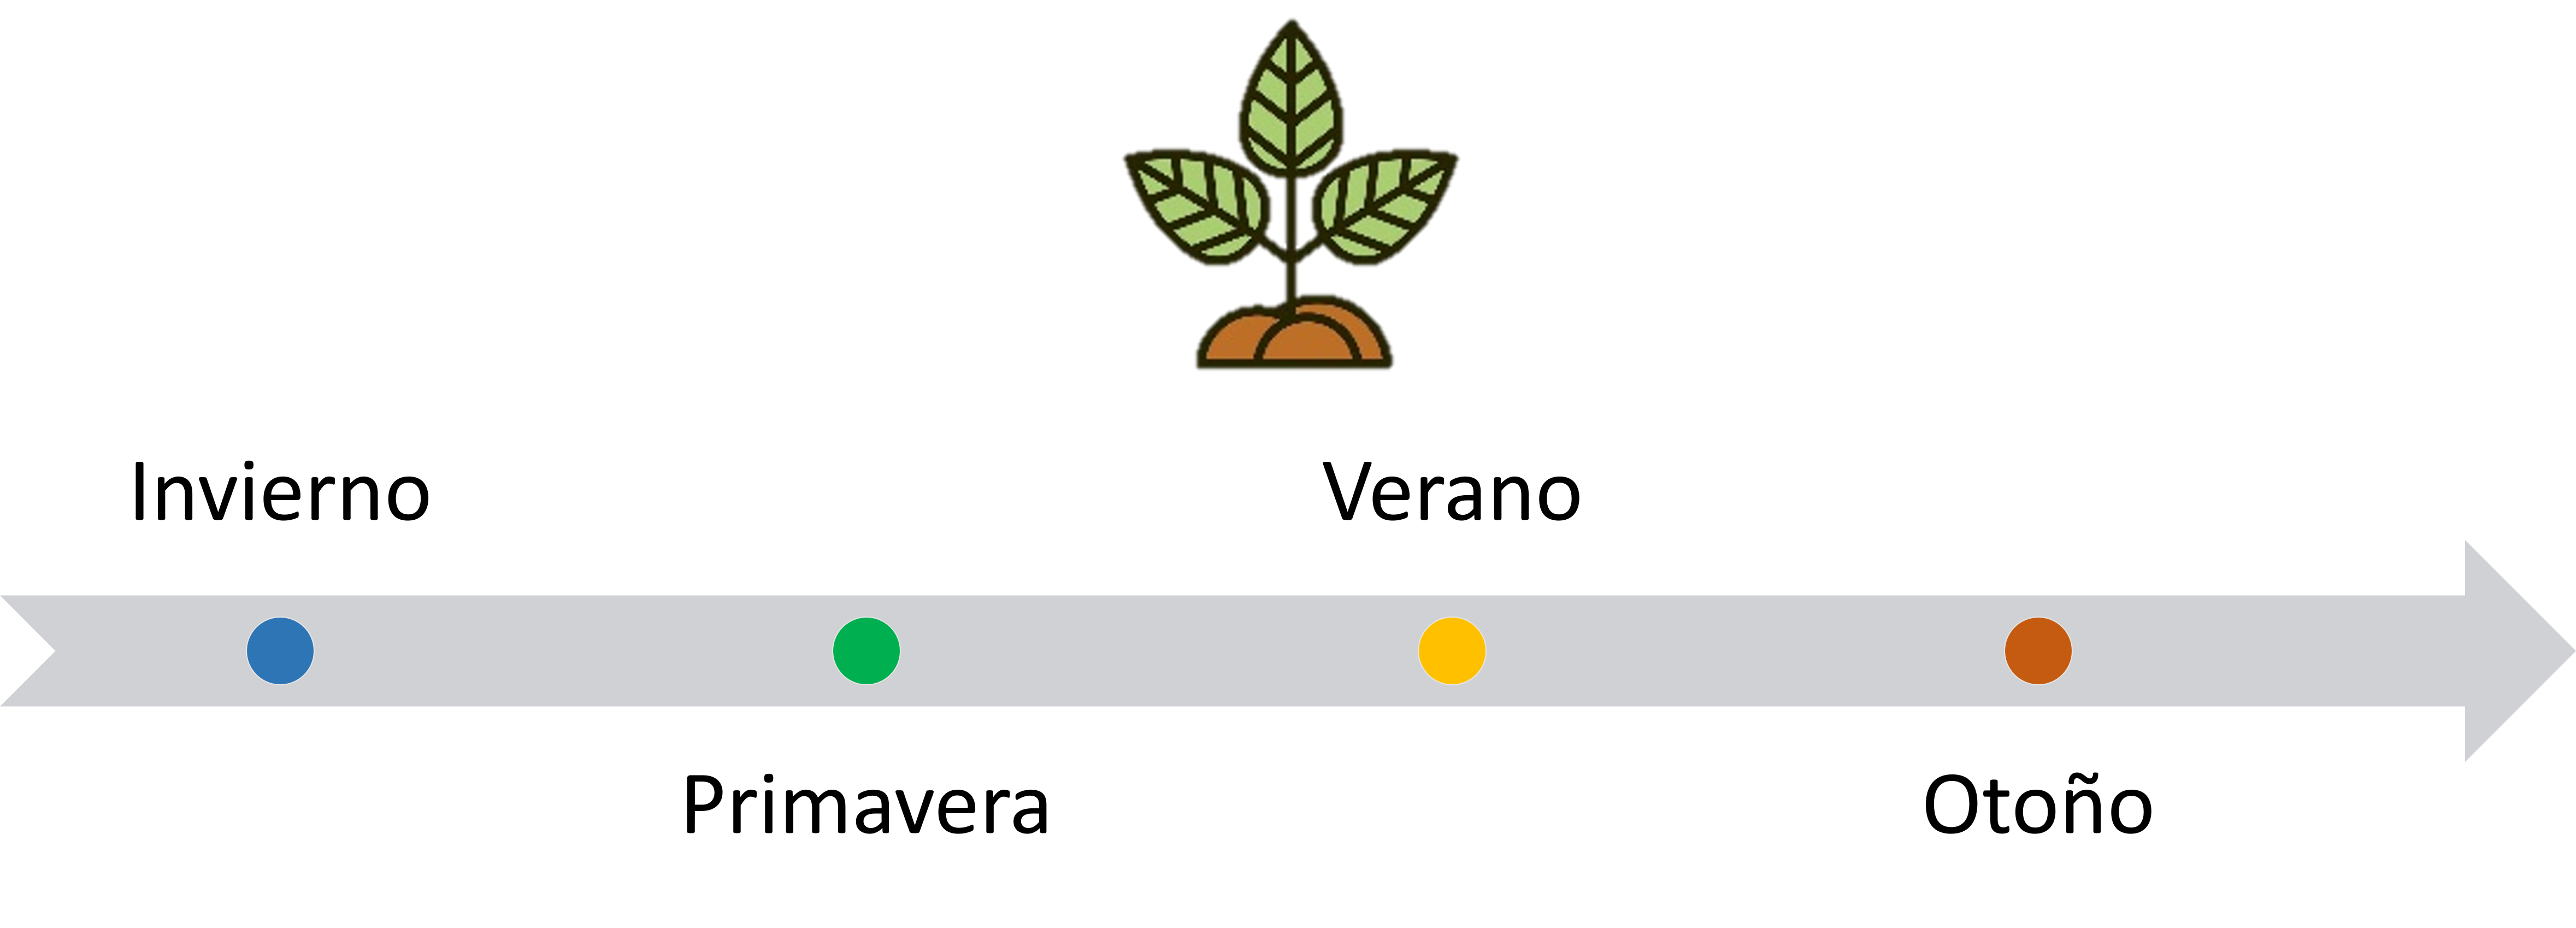
\includegraphics[width=\textwidth]{images/Choice.png}
\end{frame}

\begin{frame}{Motivación del problema}
	\vspace{-1cm}\centering
	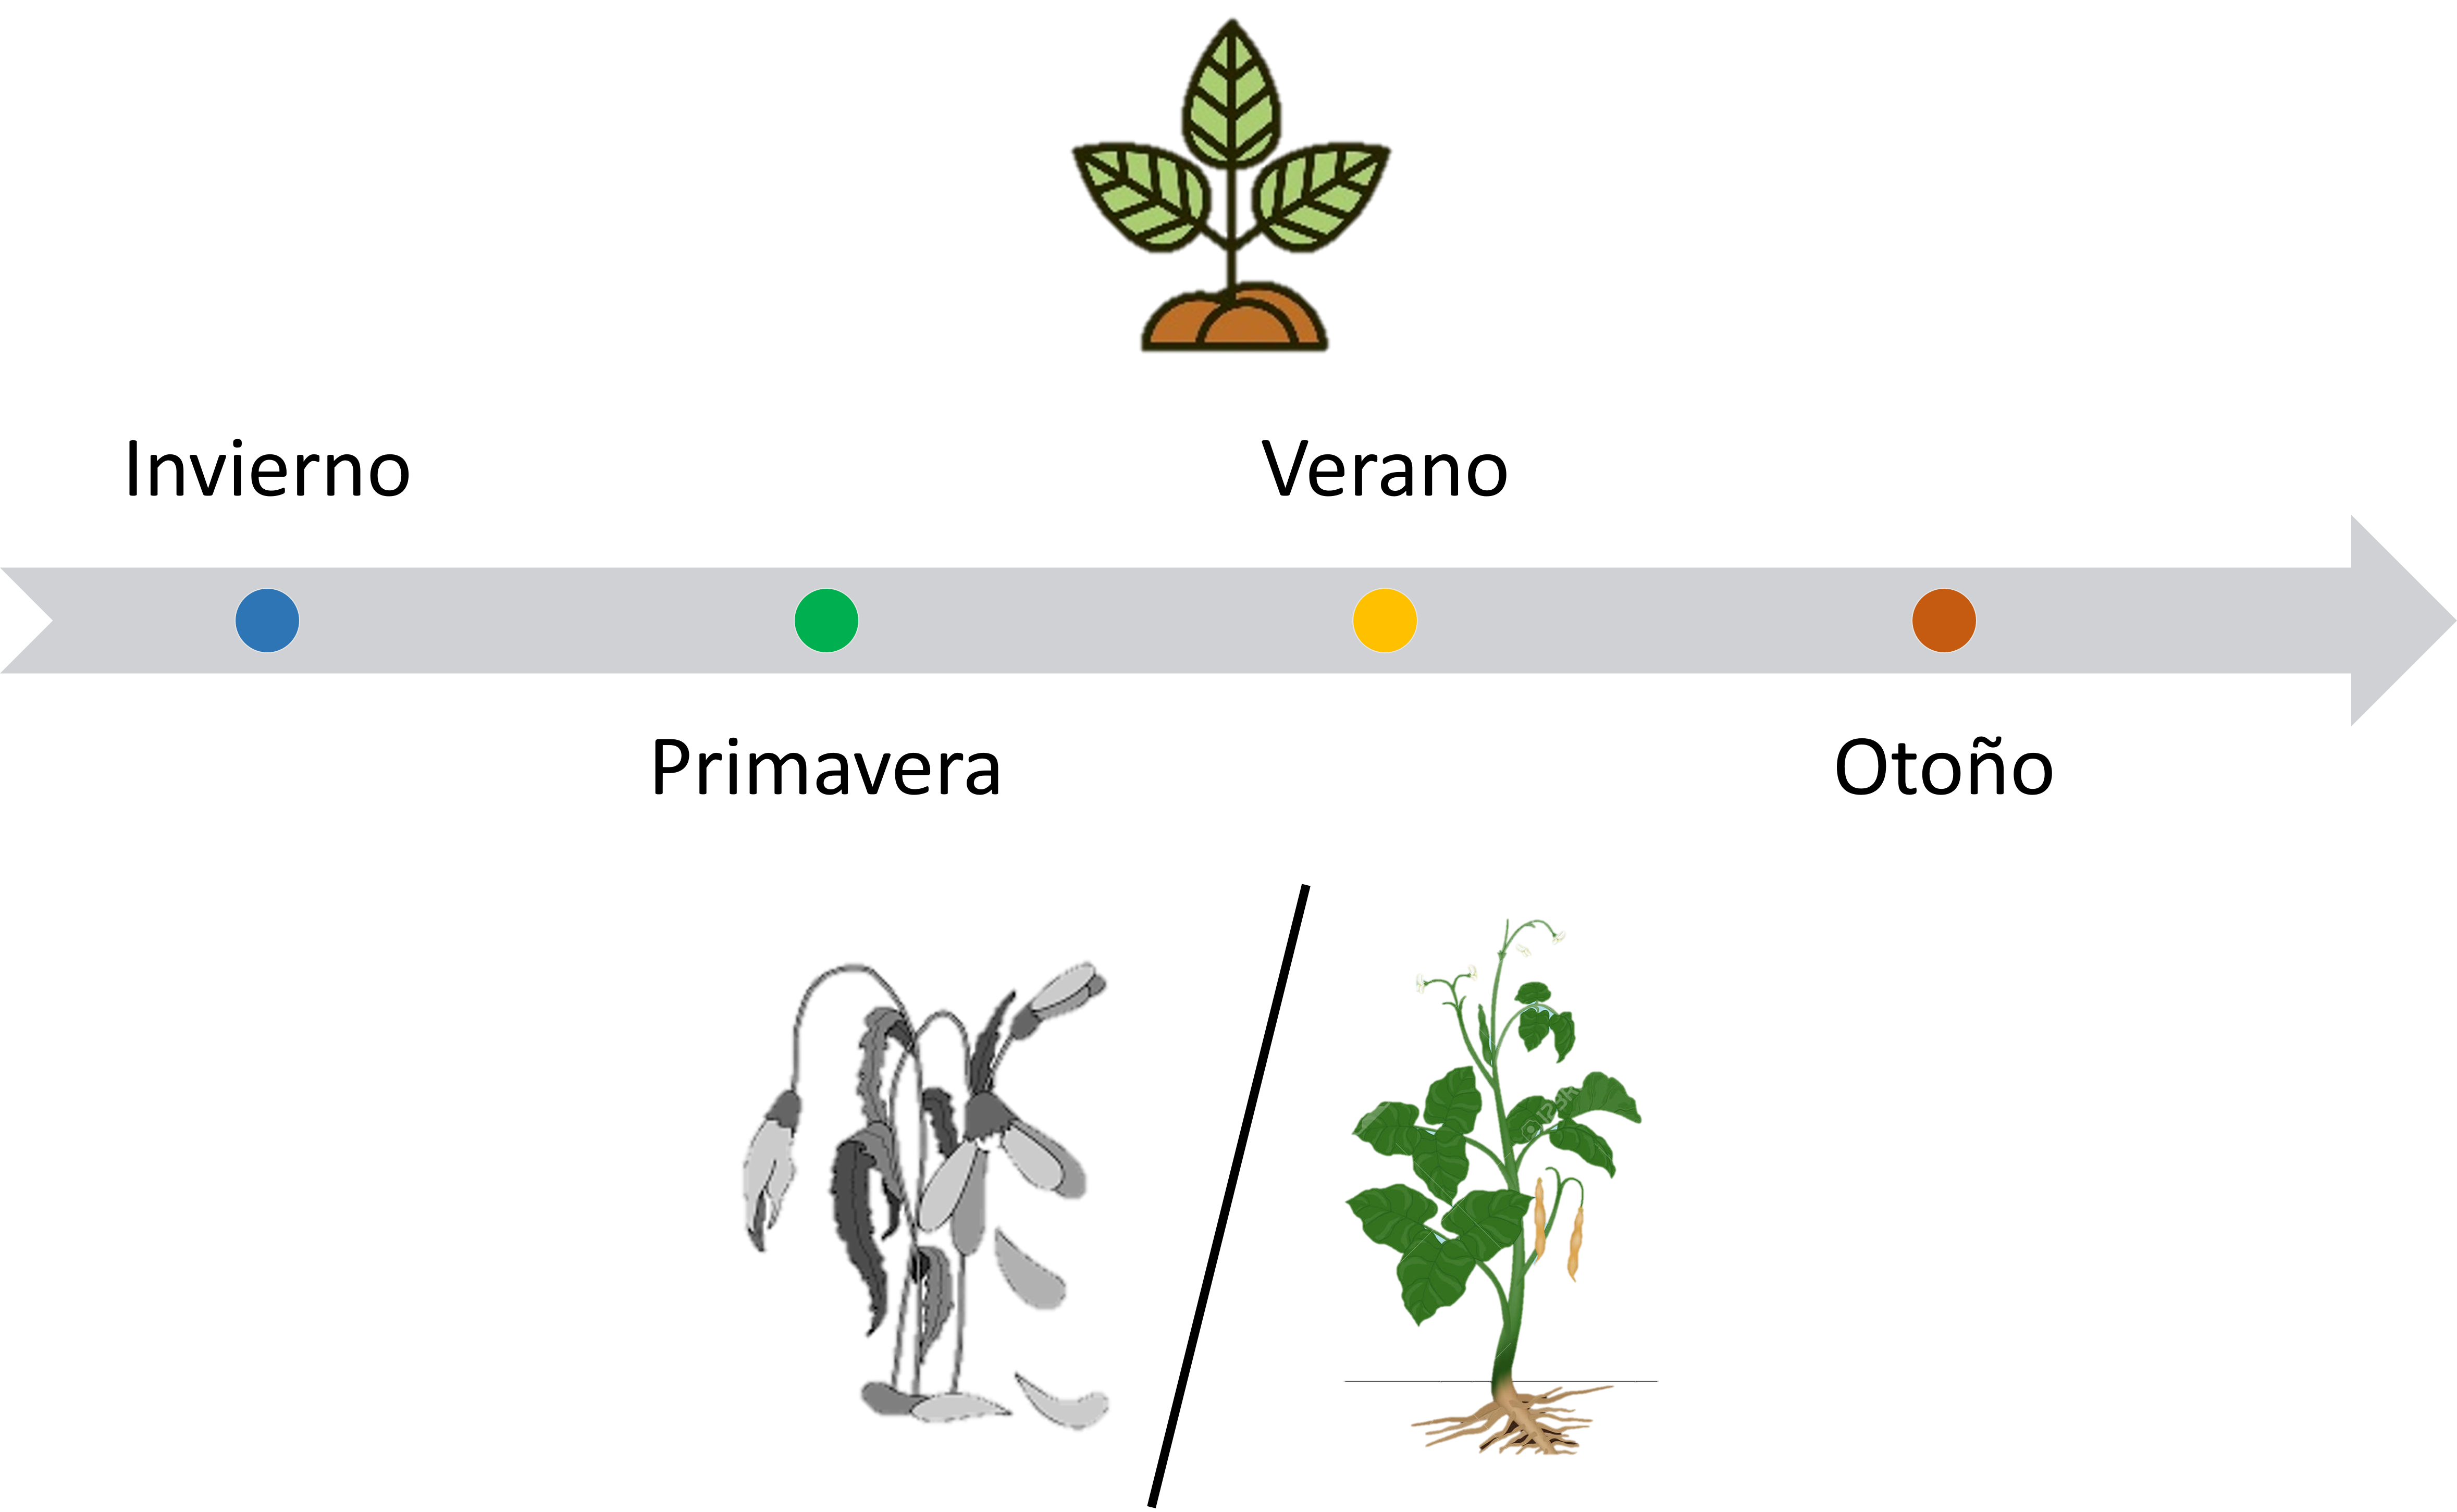
\includegraphics[width=0.9\textwidth]{images/Survival.png}
\end{frame}

\begin{frame}{Motivación del problema}
	 \vspace{-1cm}
	 \centering
	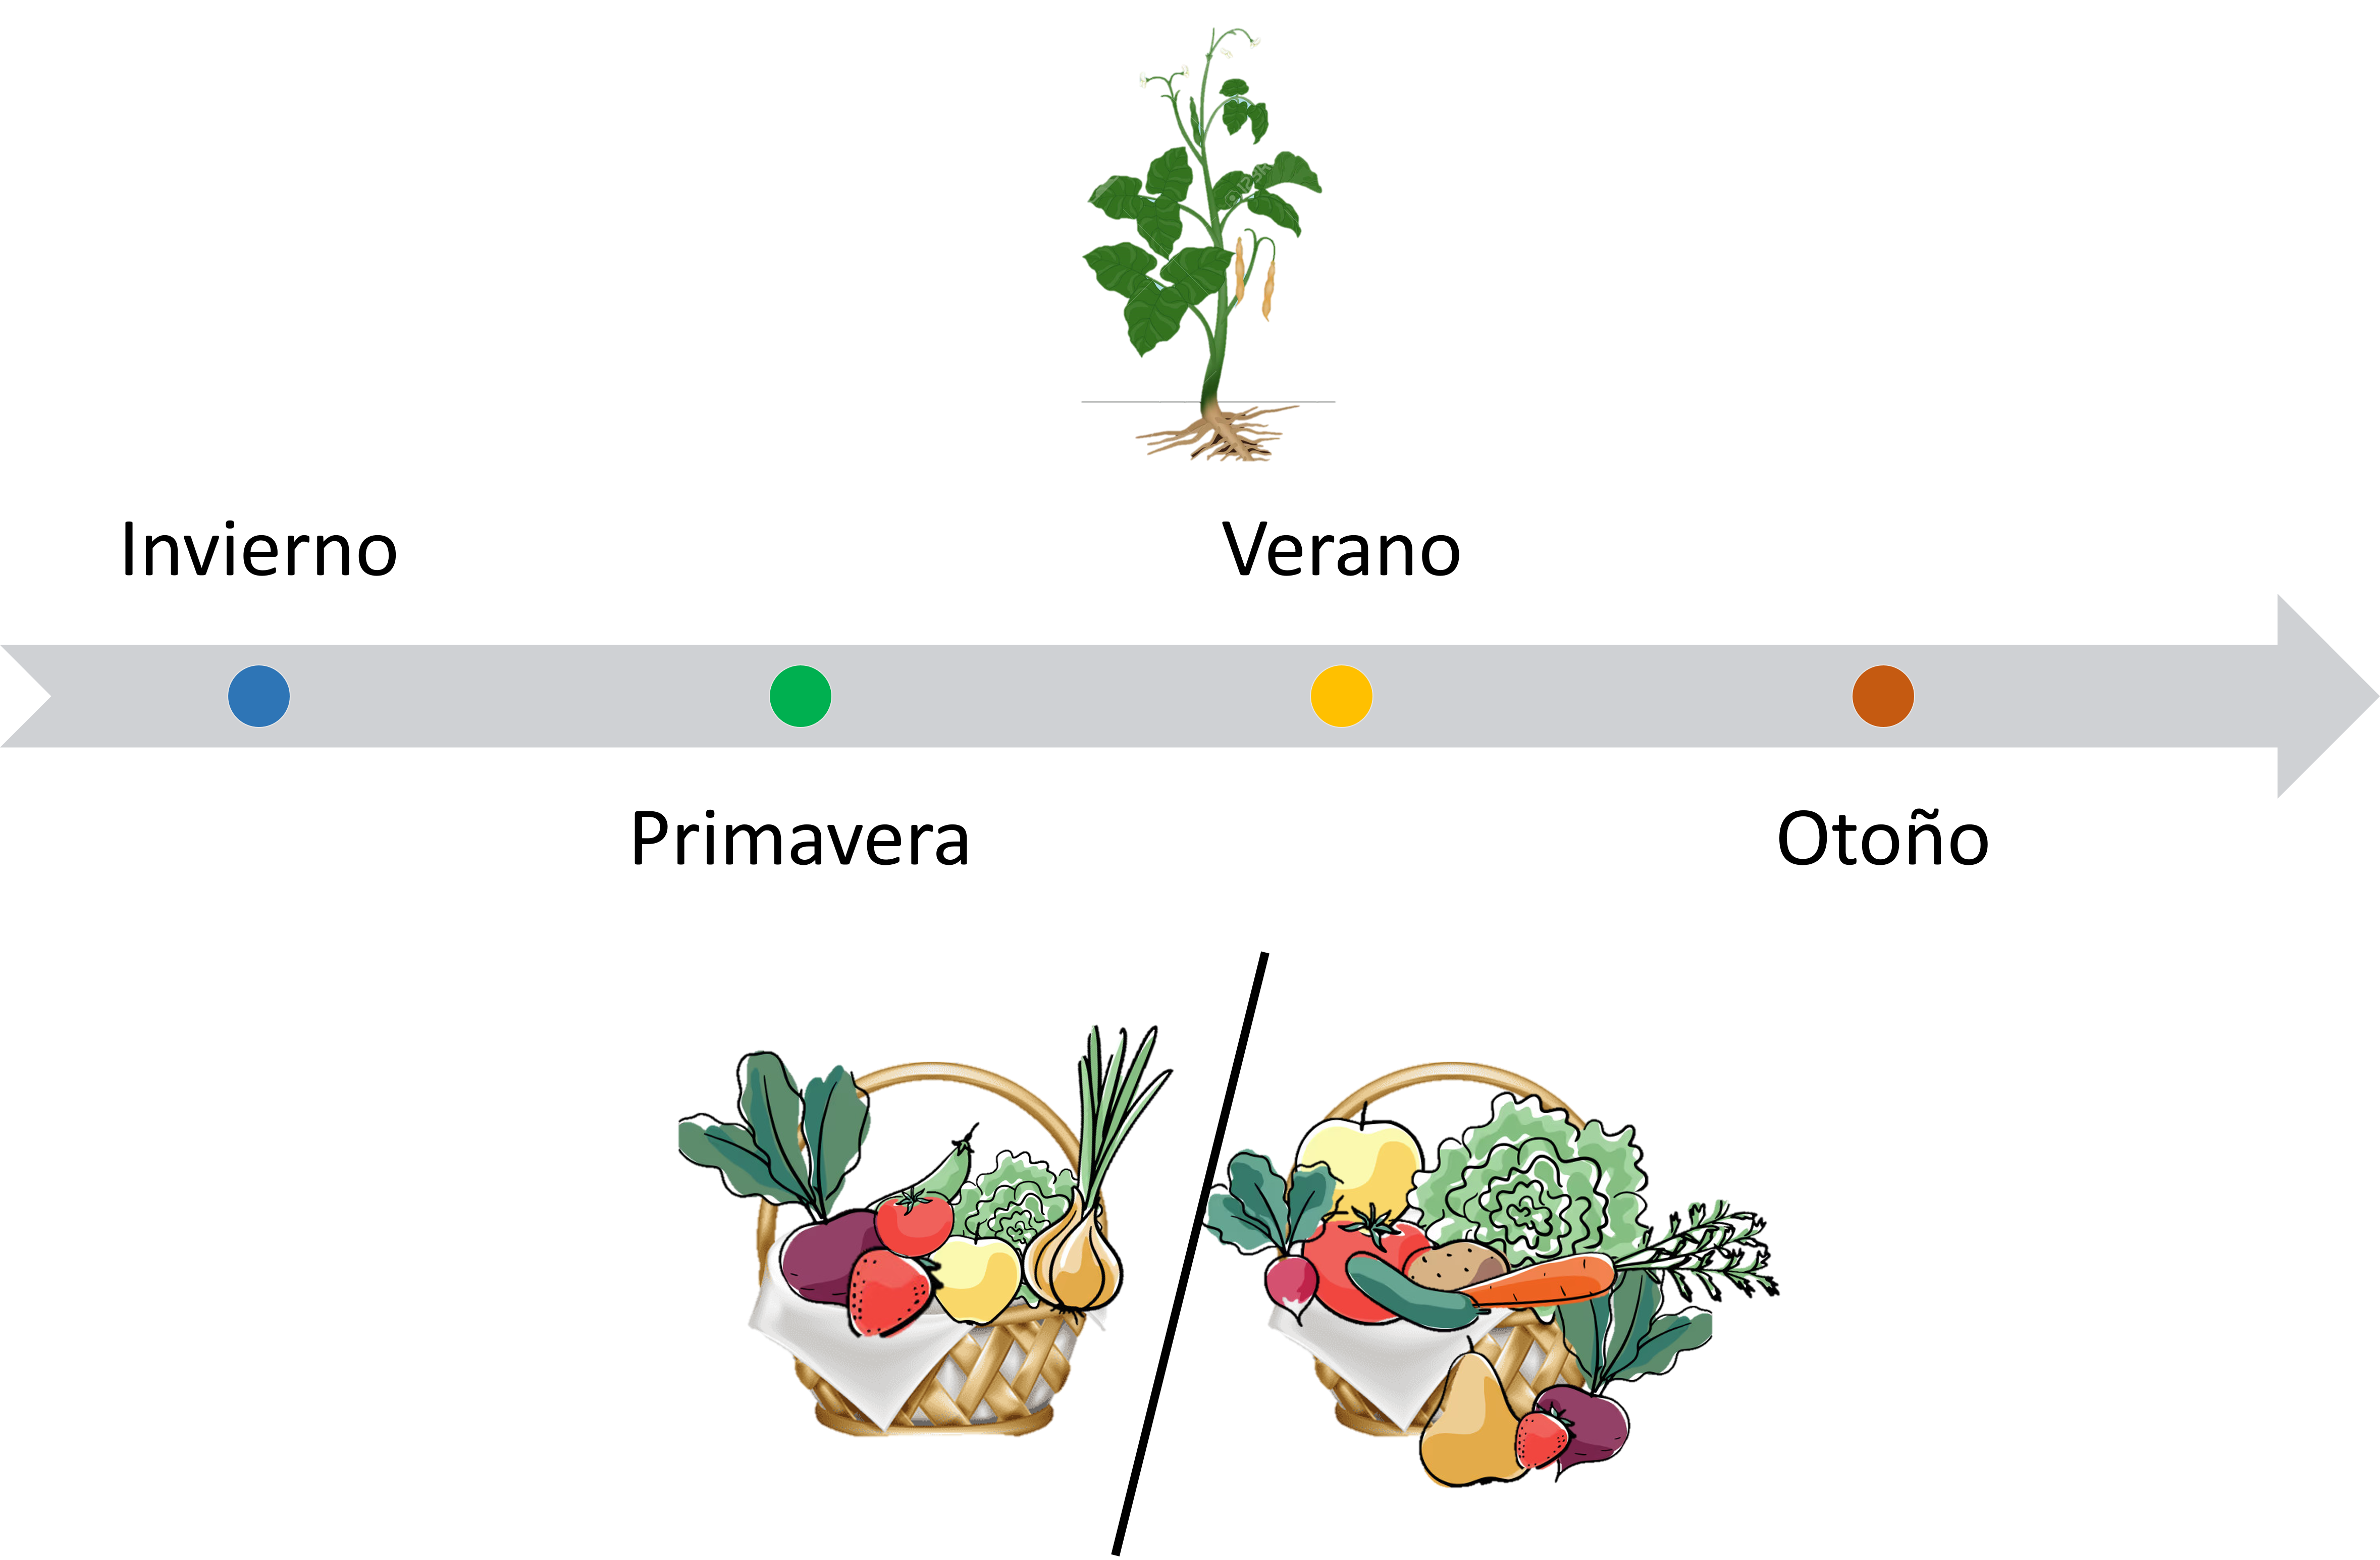
\includegraphics[width=0.9\textwidth]{images/Production.png}
\end{frame}




\begin{frame}{Impacto del cambio climático}
\vspace{-1cm}

\pause\begin{block}{\centering Consecuencias}
       \begin{minipage}{0.5\textwidth}
			\begin{itemize}
				\item Estrés ambiental.
                \item Relaciones biológicas.
			\end{itemize}
		\end{minipage}%
		\begin{minipage}{0.5\textwidth}
			\begin{itemize}
				\item Escasez laboral.
                \item Volatilidad productiva.
			\end{itemize}
		\end{minipage}
    \end{block}
    \pause
    \begin{block}{Desfase de las estaciones del año \hfill {\scriptsize Fuente: Wang \textit{et al.} (2021).}}
    \centering
        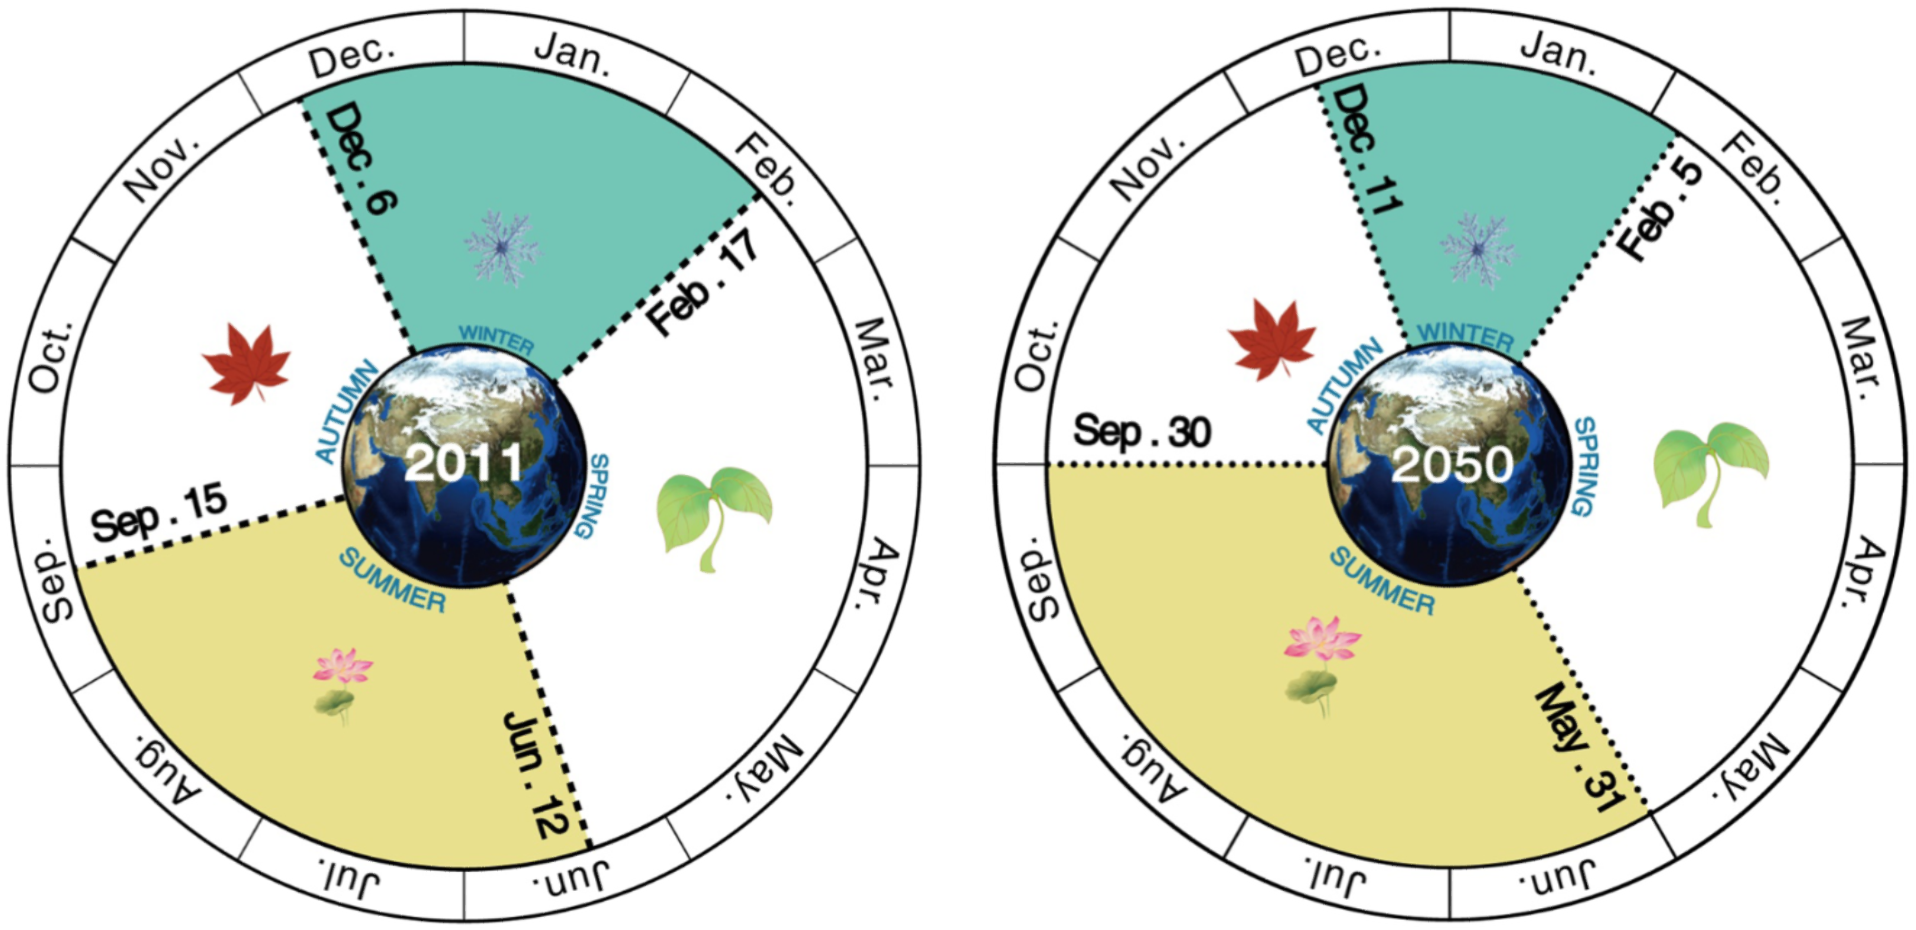
\includegraphics[scale=0.31]{images/Seasons.png}
    \end{block}
\end{frame}


\begin{frame}{El agave}
	\begin{minipage}{0.5\textwidth}
		\centering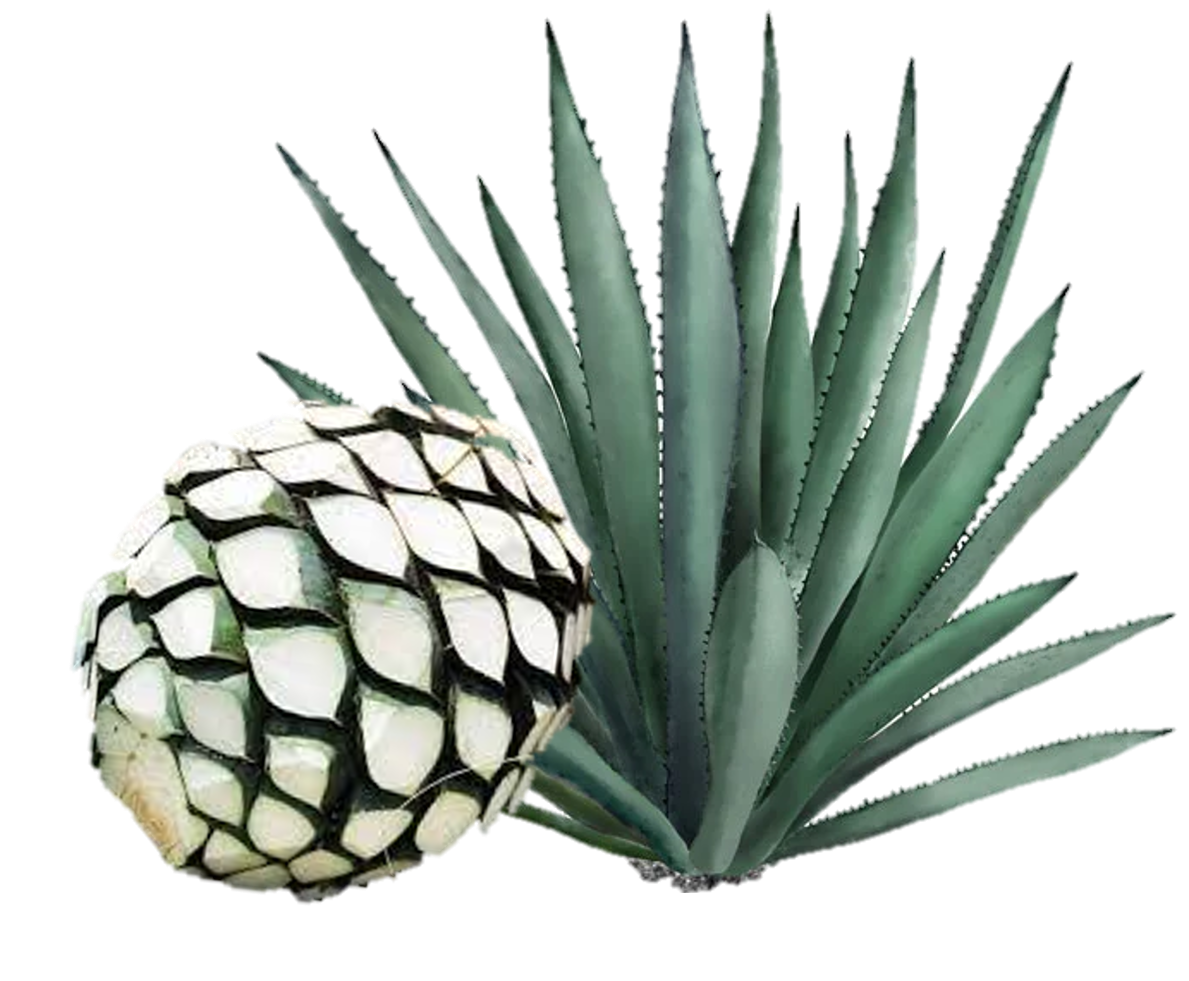
\includegraphics[width=\textwidth]{AgaveyPina.png}
	\end{minipage}%
	\begin{minipage}{0.5\textwidth}
		\begin{block}{}
			\begin{itemize}
				\item Diversidad de especies nativas.
				\item Presencia del 75\% en el territorio nacional.
				\item Aportación del 1.25\% del PIB agrícola.
				\item Tolera altas temperaturas, radiación solar y sequías.
			\end{itemize}
			 {\scriptsize Fuente: García-Mendoza, A. (2007); SAGARPA (2017);  Fernández Galicia \textit{et al.} (2023).}
		\end{block}
	\end{minipage}
	\pause\centering Se especula que será un cultivo muy rentable del futuro.\\
	{\scriptsize Fuente: Stewart, J.R. (2015).}
\end{frame}


\begin{frame}{Agave en Aguascalientes}
    \vspace{-1cm}
    \begin{minipage}{0.5\textwidth}
			\hspace{-0.5cm}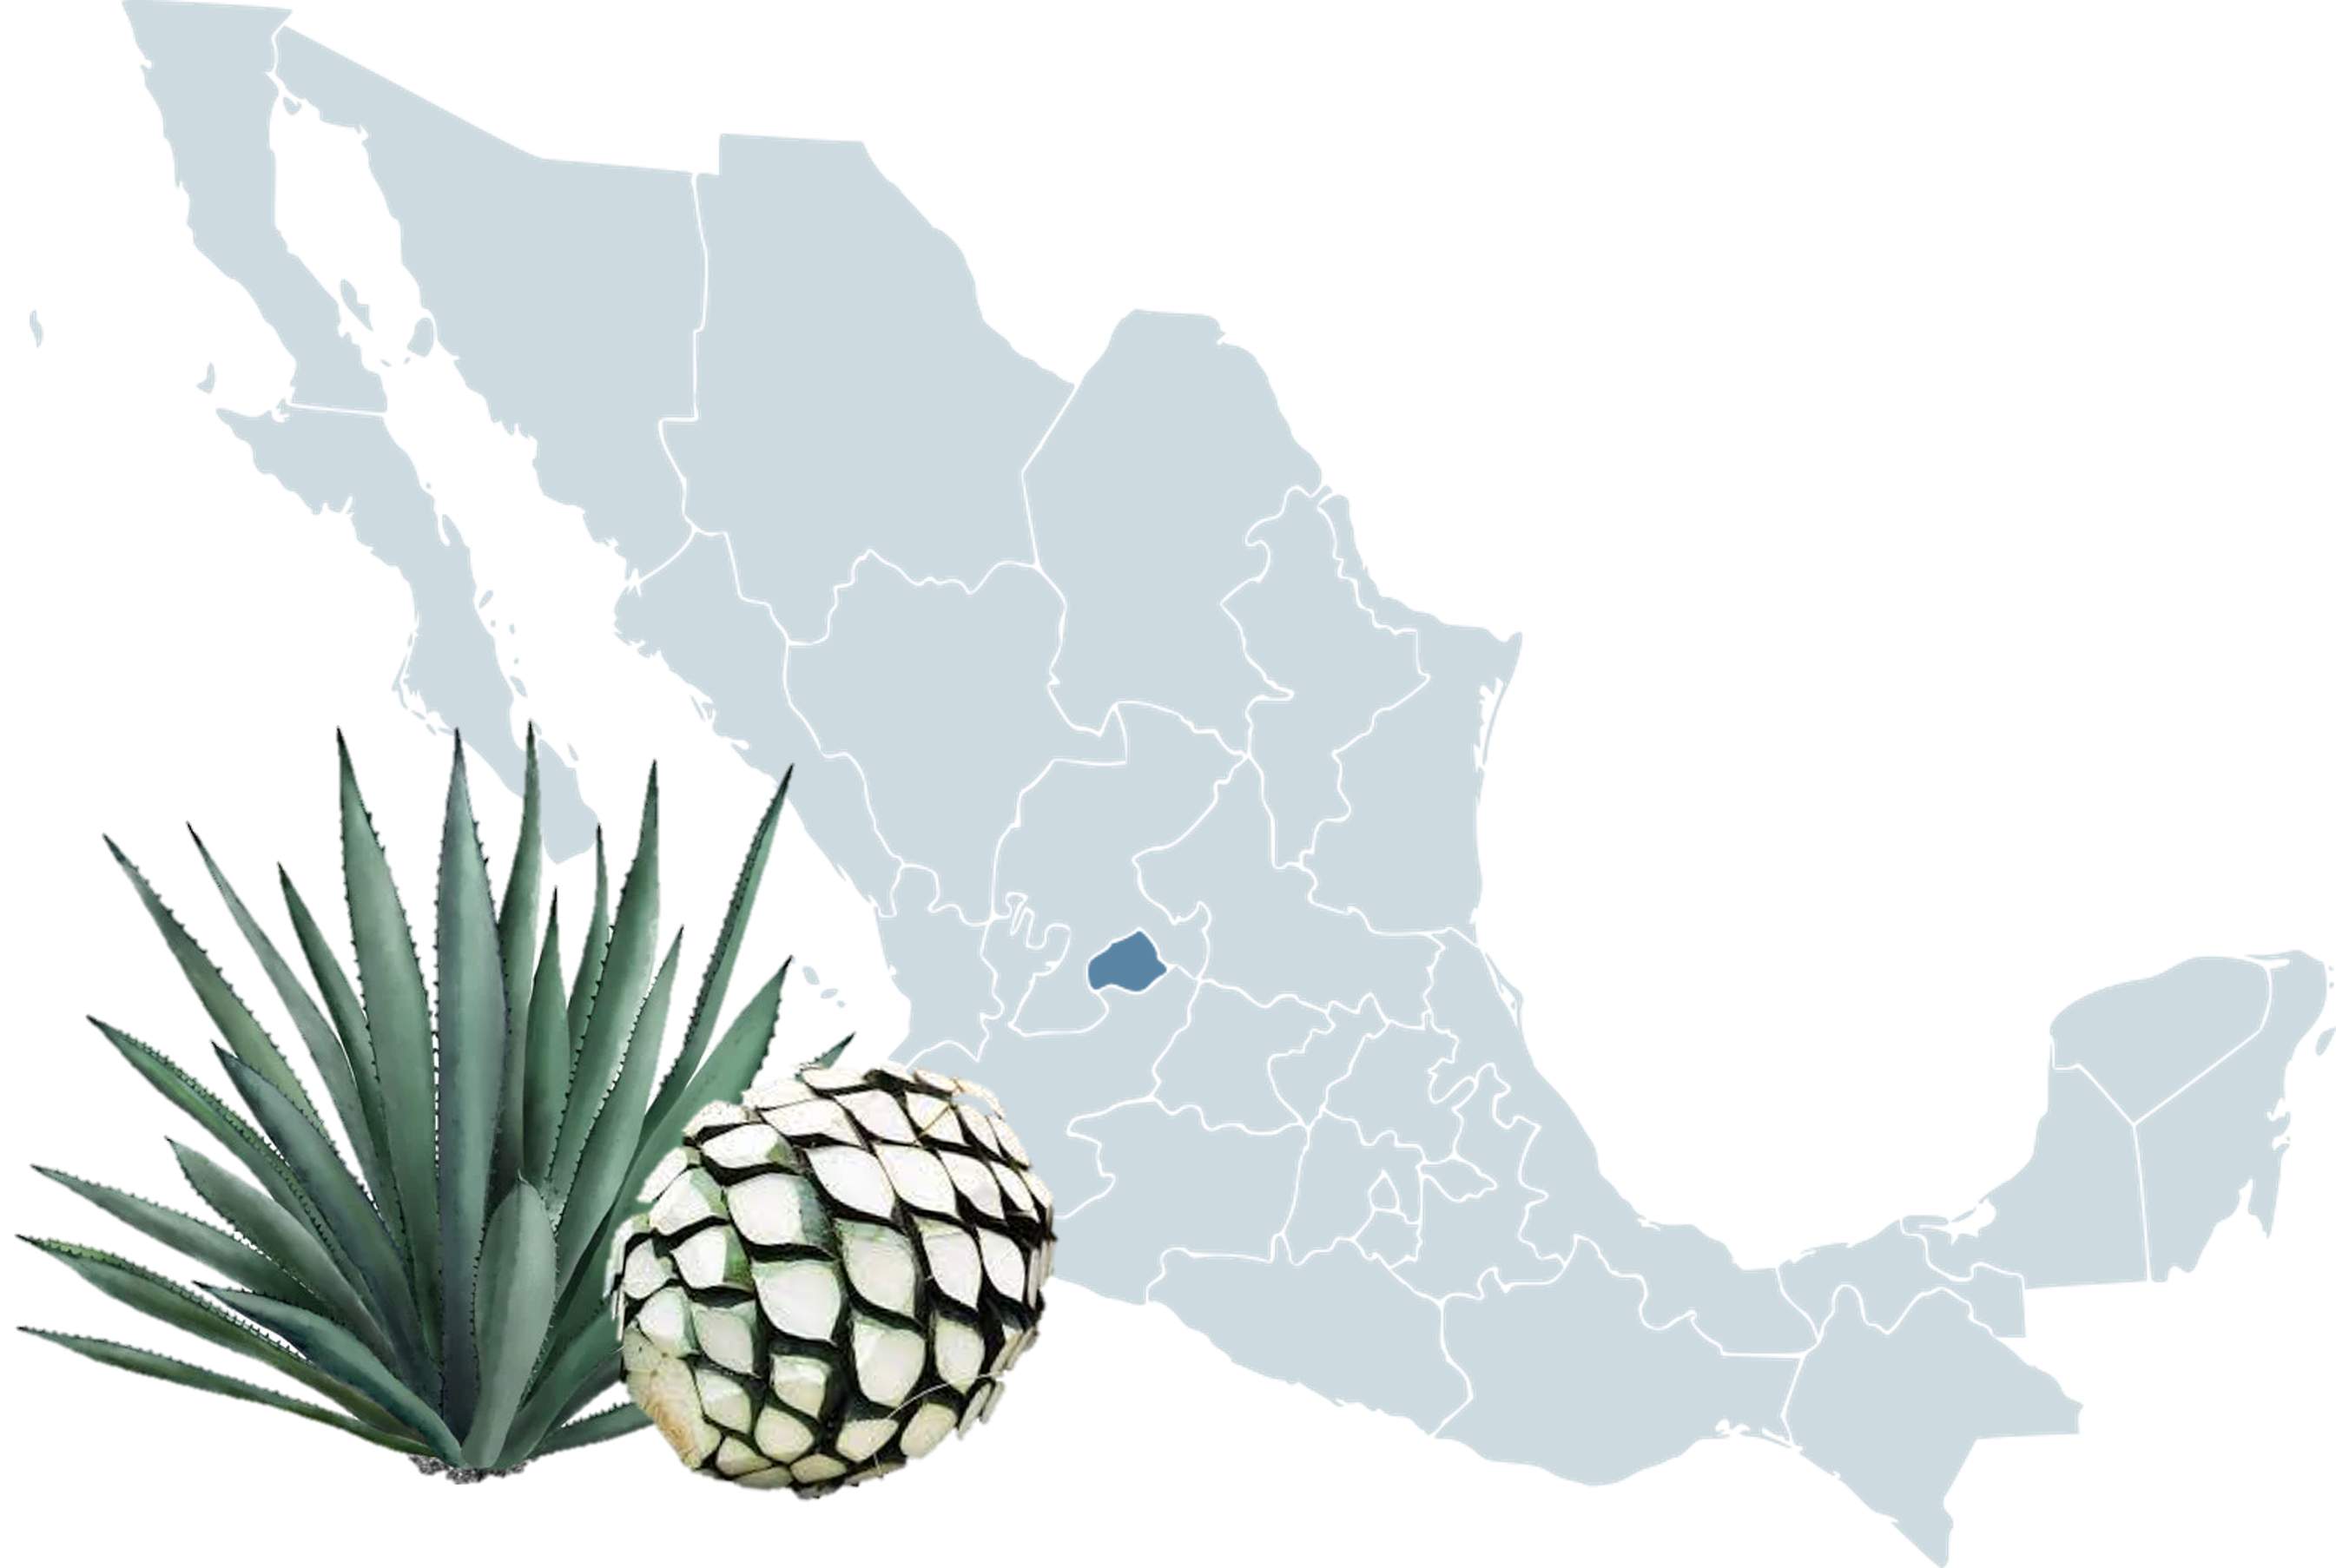
\includegraphics[width=\textwidth]{images/AgaveAGS.png}
		\end{minipage}%
		\begin{minipage}{0.5\textwidth}
			\begin{block}{Angustifolia Haw. y Salmiana Otto ex Salam-Dyck}
				\hfill {\scriptsize Fuente: Gallardo-Valdez \textit{et al.} (2019).}
			\end{block}
            \pause\begin{block}{Requerimientos}
                \begin{itemize}
				\item Suelos con pH de 6 -- 7 y profundidades de, al menos, 1 m.
                    \item Precipitaciones anuales de 600 mm. uniformemente distribuidas.
                    \item Ausencia de heladas.
                    \item Altitudes máximas de 2000 m.s.n.m.
                    \item Temperaturas de -5$^\circ$ C -- 45$^\circ$ C. 
			\end{itemize}
            \end{block}
		\end{minipage}
        \,\\
        \hfill {\scriptsize Fuente: CONAFOR (s.f.);  Fernández Galicia \textit{et al.} (2023).}
\end{frame}


\begin{frame}{Agave en Aguascalientes}
	\vspace{-1cm}
	\begin{minipage}{0.5\textwidth}
		\begin{block}{Productos}
			\begin{itemize}
				\item Bebidas.
				\item Aditivos alimenticios.
				\item Textiles básicos.
				\item Pomadas.
				\item Envases desechables.
			\end{itemize}
			{\scriptsize Fuente: Alonso-Tapia, H. (2022).}
		\end{block}
	\end{minipage}%
	\begin{minipage}{0.5\textwidth}
		\centering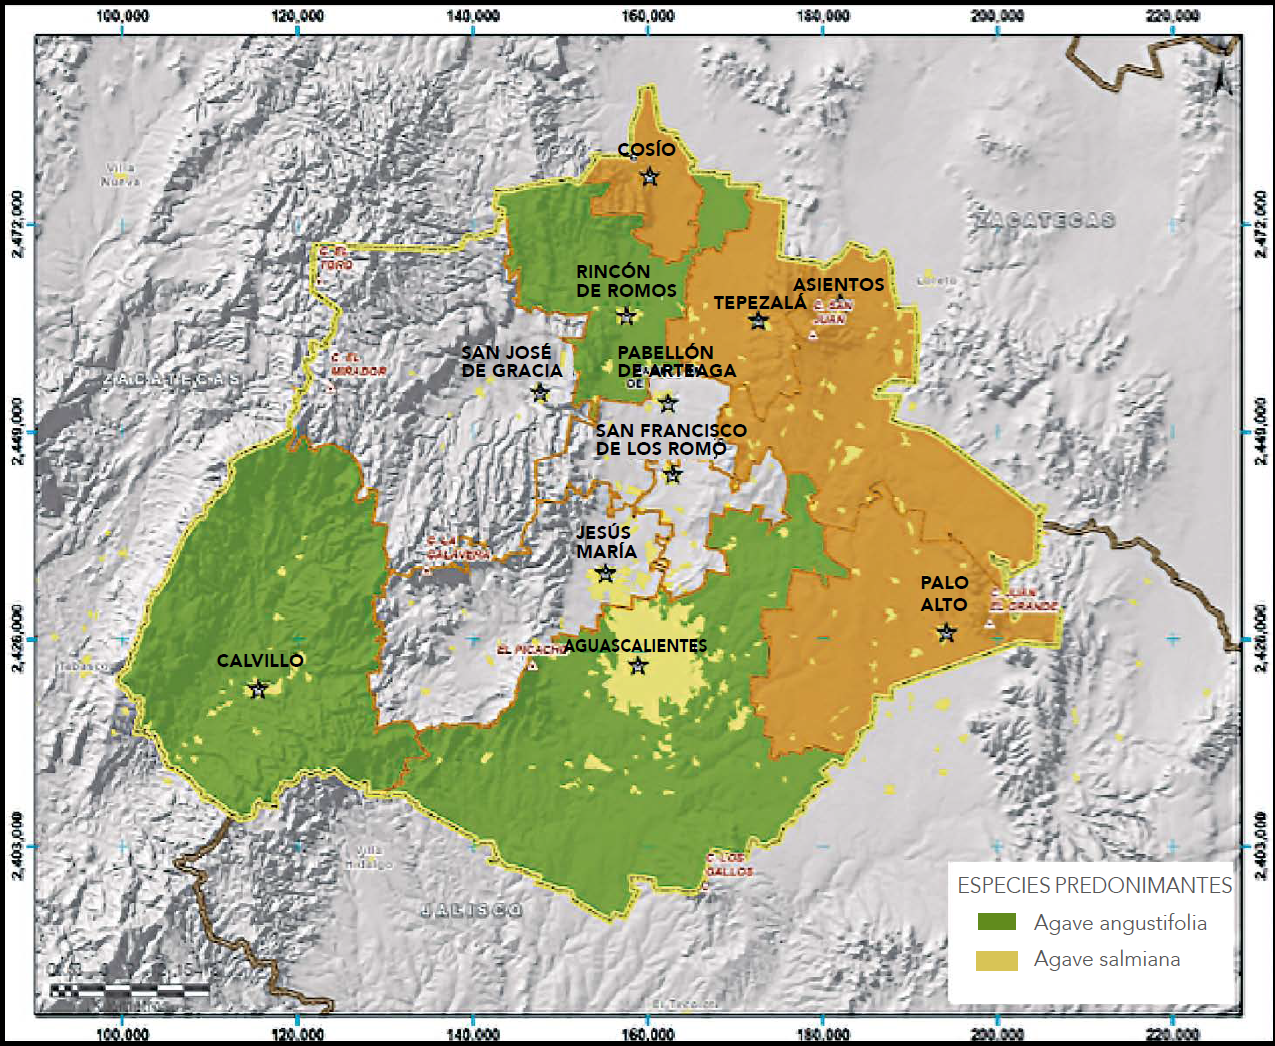
\includegraphics[height=0.73\textheight]{images/DistribucionAGS.png}\\\hfill {\scriptsize Fuente: CIATEJ (2016).}
	\end{minipage}%
\end{frame}


\begin{frame}{Agave en Aguascalientes}
	\vspace{-1cm}
	\begin{minipage}{0.5\textwidth}
		\begin{block}{Usos potenciales}
			\begin{itemize}
				\item Biocombustible.
				\item Bioinsecticidas.
				\item Prebióticos.
				\item Medicamentos.
				\item Textiles complejos.
				\item Papel.
				\item Alimento para animales.
				\item Fitoremediación.
			\end{itemize}
			{\scriptsize Fuente: Stewart, J.R. (2015); Fernández-Galicia, \textit{et al}. (2024).}
		\end{block}
	\end{minipage}%
	\begin{minipage}{0.5\textwidth}
		\centering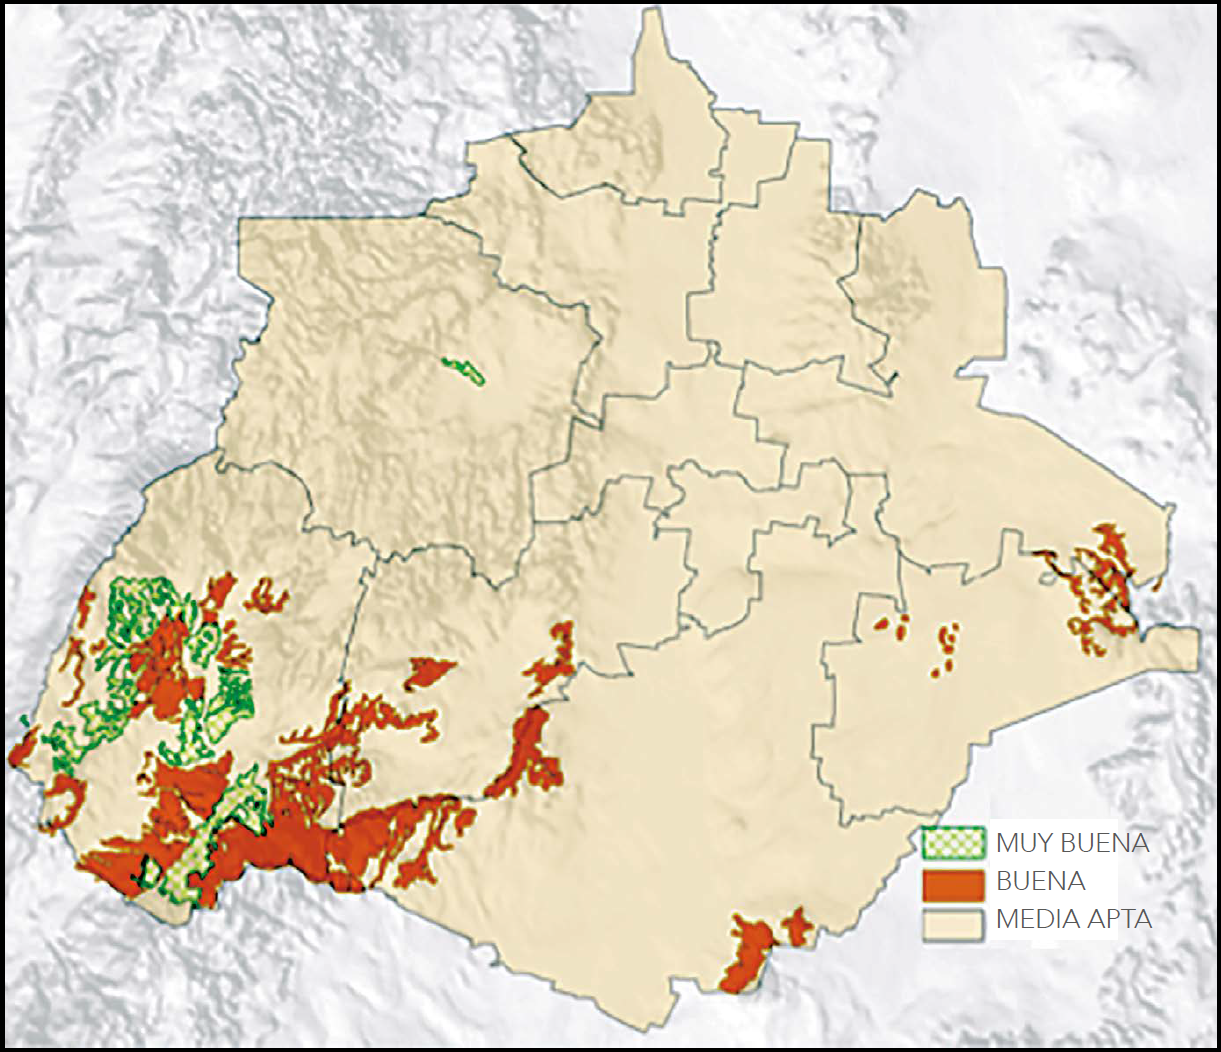
\includegraphics[height=0.73\textheight]{images/AptitudAGS.png}\\\hfill {\scriptsize Fuente: INIFAP (2002).}
	\end{minipage}%
\end{frame}

\section{¿Qué queremos?}
\begin{frame}{Fechas de trasplante}
	\begin{minipage}{0.5\textwidth}
		\hspace{-0.5cm}
		\centering
		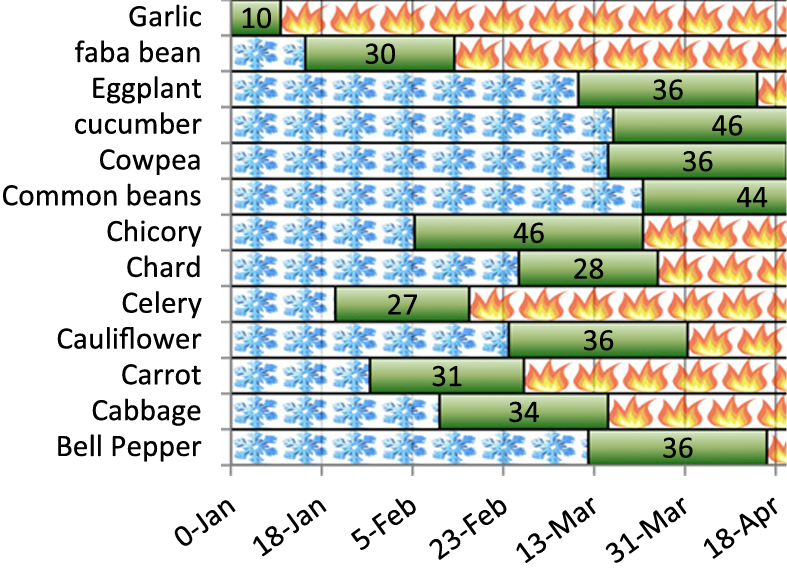
\includegraphics[width=\textwidth]{images/Elnesr.png}
		{\scriptsize Fuente: Elnesr \textit{et al.} (2013).}
	\end{minipage}%
	\begin{minipage}{0.5\textwidth}
		\vspace*{-2cm}\begin{block}{}
			Determinar periodos ideales.\\ 
			\pause Maximicen tasa de supervivencia.\\
			Reduzcan pérdidas económicas.
		\end{block}
	\end{minipage}
\end{frame}


\begin{frame}{Estimar la materia prima}
	\begin{minipage}{0.5\textwidth}
		\vspace*{-1cm}\begin{block}{}
			Calcular el peso fresco/seco.\\ 
			A gran escala.\\
			Incluyendo plantas de distintas edades.
		\end{block}
	\end{minipage}%
	\begin{minipage}{0.5\textwidth}
		\hspace{-0.5cm}
		\centering
		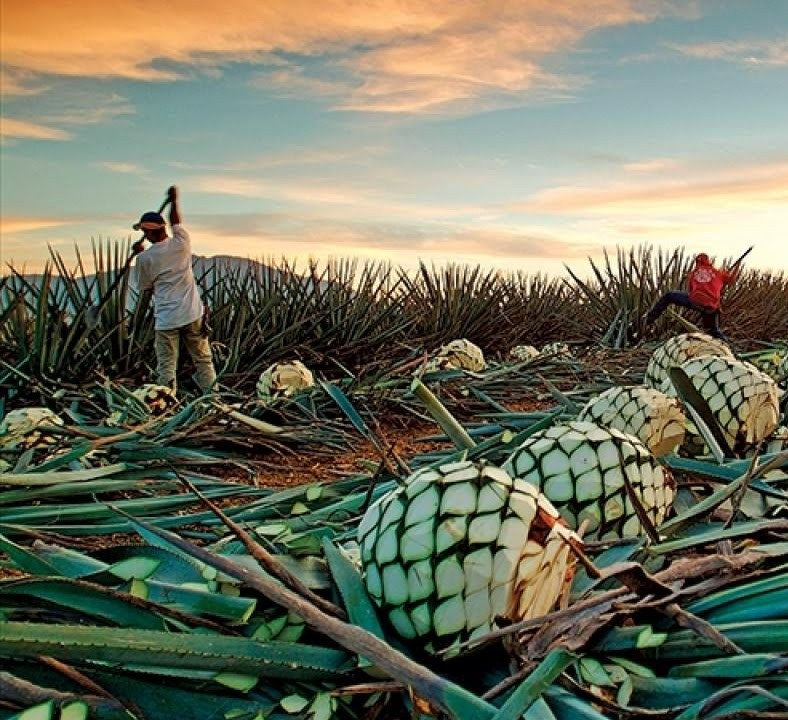
\includegraphics[width=\textwidth]{images/Biomass.jpg}
	\end{minipage}
\end{frame}

\section{¿Qué ganamos?}

\begin{frame}{Beneficios}
	\begin{block}{}
		\begin{itemize}
			\item Facilitar el proceso de plantación.
			\item Reducir la muerte de las plantas.
			\item Favorecer el desarrollo del cultivo.
			\pause \item Conocer, de antemano, el peso de la cosecha.
			\item Estimar el valor comercial y ganancias.
		\end{itemize}
	\end{block}
\end{frame}

\section{¿Qué necesitamos?}

\begin{frame}{Datos}
	\begin{minipage}{0.5\textwidth}
		\vspace*{-1cm}\begin{block}{}
			Ubicación de parcelas.\\
			Variedad que siembran.\\
			Edades de los agaves.\\
			Producción de +5 ciclos productivos.\\
			Número de productores.\\
			Manejo agrícola.\\
			Fechas de siembra.\\
			Tipos de suelo.
		\end{block}
	\end{minipage}%
	\begin{minipage}{0.5\textwidth}
		\vspace{-0.5cm}
		\centering
		
\includegraphics[width=\textwidth]{images/QR_code.png}
	\end{minipage}
\end{frame}

\section*{Referencias}
\begin{frame}[allowframebreaks,noframenumbering]{Referencias}
	\vspace*{-1cm}
	\tiny
	\bibliography{BibliografiaUP.bib}
	\bibliographystyle{alpha}
	\nocite{*}
	%\printbibliography
\end{frame}

\section*{Gracias}
\begin{frame}[noframenumbering]
%\vspace{2cm}
     \begin{center}
	    \Huge{Gracias}
	\end{center}
    \end{frame}
    
    
 \begin{frame}{}
 	 \begin{block}{Métodos}
 		\begin{itemize}
 			\item Algoritmos de decisión simple.
 			\item Modelos de suavizamiento exponencial.
 			\item Redes neuronales recurrentes.
 			\item Regresiones.
 			\item Perceptrón multicapa.
 			\item Support vector machine.
 			\item Árboles de decisión.
 			\item Bosques aleatorios.
 			\item k vecinos más cercanos.
 			\item M5 Prime.
 		\end{itemize}
 	\end{block}
 \end{frame}
\end{document}
